% Yes, I have not followed two of the requirements specified in the style guide: the paragraph indenting and the exact style of referencing. My reasons are. Both are very difficult to set up in LaTeX and I have not seen either style used in any academic mathematics paper which I have read. My choice of indenting (the default by LaTeX) still distinguishes the start of paragraphs, while my referencing contains all required information and in-text citations follow Havard style.



\documentclass[a4paper, fontsize=12pt]{article}
\usepackage{macros-ohp}
\usepackage{LBlake_style}

\usepackage[nottoc]{tocbibind}

\usepackage{algorithm}
\usepackage{natbib}
\setcitestyle{authoryear,open={(},close={)}}
\usepackage[title]{appendix}

\usepackage{wrapfig}

%Please make sure the tex is compiled twice to have all the background images displayed correctly.

\title{\Huge \textbf{Identifying Lagrangian Coherent Structures with Fuzzy Consensus Clustering}}

\author{\Huge Liam Blake\\
	\Large Supervised by Associate Professor Sanjeeva Balasuriya \& Dr. John Maclean\\
	\Large The University of Adelaide\\
}
\date{}

\linespread{1.5}

\renewcommand{\sc}{;\,}
\newcommand{\ddeg}{^{\circ}}

\renewcommand{\floatpagefraction}{.8}%

\begin{document}
	\begin{titlingpage}
	\tikz[remember picture,overlay] \node[opacity=1,inner sep=0pt] at (current page.center){\includegraphics[width=\paperwidth,height=\paperheight]{imgs/background.png}};
	\vspace*{3.5cm}
	{\let\newpage\relax\maketitle}
	\vspace*{\fill}
	\begin{textblock*}{140mm}(40mm,200mm)
			\begin{center}
				\begin{small}
		
Vacation Research Scholarships are funded jointly by the Department of Education, Skills and Employment
and the Australian Mathematical Sciences Institute.

				\end{small}
			\end{center}
	\end{textblock*}

	\end{titlingpage}




\section*{Abstract}
Lagrangian coherent structures are moving entities within a fluid flow that produce coherent and observable patterns in the flow. These can be extracted by grouping trajectories into coherent regions or partitions. There are many different methods for defining and extracting these regions, with no unifying framework which can merge different structures into one partitioning of a flow. 

This paper proposes a clustering framework to allow comparison of coherent regions obtained from differing approaches. Fuzzy clustering generalises clustering to membership values, which can better distinguish cluster boundaries and outliers. Moreover, consensus clustering provides a family of robust algorithms for combining multiple clusterings of the same data into one. We explore the application of fuzzy consensus clustering (FCC), which is one such algorithm, on current velocity and sea surface temperature measurements taken from the Atlantic Ocean and including part of the Gulf Stream. We first perform an LCS analysis of this data, using several different techniques, then combine the resulting partitions with the FCC algorithm. This approach was shown to provide a promising foundation by being able to improve individual results and extract new structure from the flow.


%\vspace{5mm}


\section{Introduction}
In many fluid flows, there are regions of coherency that are transported by the flow, e.g. vortices and flow barriers. By defining and extracting these regions mathematically, we can gain more insight into material transport by the flow. These regions are often seen in experimentally observed flows, such as Agulhas rings which transfer heat and salt concentration between the Indian and Atlantic oceans, and have many applications including drifter tracking and forecasting. The field of Lagrangian coherent structures is concerned with extracting these regions from a given flow via a rigorous approach. These structures are extracted from particle trajectories, i.e. the Lagrangian description of the flow. There is a diverse range of techniques developed for this purpose, drawing from many different areas of mathematics. However, as a consequence of this diversity, there is no framework which unifies LCSs and allows for the combination of different structures identified in a flow.

A clustering framework is proposed to compare partitions of Lagrangian trajectories derived using different methods. Fuzzy consensus clustering (FCC) then provides a robust algorithm for combining these partitions into one. An application of this framework and consensus clustering algorithm is investigated via oceanographic measurements of part of the Gulf Stream in the Atlantic Ocean. When clustering was applied to the sea surface temperature field, the Gulf Stream was highlighted as a cluster and a flow barrier, which provided a promising and clear picture of the flow. The FCC algorithm was able to improve clusters produced using only the trajectories, by combining these with the temperature partitions Combining non-overlapping clusters with FCC gave the obvious result, where each individual cluster was included in the final partitioning. When all four basic partitions were combined, the resulting clusters were unable distinguish smaller-scale structure highlighted by FTLE and LAVD analysis. This was likely due to an insufficient number of clusters, which highlighted the need for a method to determine the optimal number of clusters which is better suited for coherent structure identification. 


 



\subsubsection*{Statement of Authorship}
LB formulated the clustering framework, acquired the data, wrote the \textsc{Matlab} code and produced and interpreted results. SB provided the initial project formulation and ongoing guidance. JM provided additional guidance, and proof-read and provided feedback on this report.


\section{Background}
\subsection{Mathematical Set-Up}
Consider some open connected subset \(\Omega \subset \R^d\) (where \(d\) is usually 2 or 3) called the flow domain, and some finite time interval \([-T,T]\) of interest. The fluid velocity at a fixed point in space and time is given by the Eulerian velocity field \(\bm{v}:\Omega\times[-T,T] \to \R^n\), which we assume to be sufficiently smooth such that \(\bm{v} \in \mathcal{C}^1(\Omega\times(-T,T))\) to ensure existence and uniqueness of trajectories. We assume that \(\bm{v}\) is known, or at least can be numerically or empirically approximated.

The trajectory beginning at position \(\bm{x}_0 \in \Omega\) at initial time \(t_0 \in [-T,T]\) is the unique solution \(\bm{x}(t; \bm{x}_0)\) to
\begin{equation}
\dot{\bm{x}} = \bm{v}(\bm{x},t); \quad \bm{x}(t_0) = \bm{x}_0.
\label{eqn:trajode}
\end{equation}

The trajectories are summarised by the flow map \(F_{t_0}^{\cdot}: \Omega \times [-T,T] \to \R^2\) which arises as the solution to
\begin{equation}
\dpd{F_{t_0}^{s}(\bm{x}_0)}{s} = \bm{v}\left(F_{t_0}^s(\bm{x}_0), s\right),
\label{eqn:flowmap}
\end{equation}
and satisfies \(F_{t_0}^{t_0}(\bm{x}_0) = \bm{x}_0\). The flow map is the mapping from initial particle positions to their later positions, i.e. \(F_{t_0}^{t}: \bm{x}_0 \mapsto \bm{x}(t;\bm{x}_0)\).


\subsection{Lagrangian Coherent Structures}
In a flow fluid, \textit{coherency} refers to observable patterns within a flow or regions of flow that remain similar in some way over some time-interval. A specific class of coherent structures that have received significant interest are \textit{Lagrangian coherent structures} (LCSs). These are coherent entities associated with the individual particle trajectories of a flow satisfying \eqref{eqn:trajode}. LCSs can be considered generalisations of easily identifiable coherent flow structures, such as vortices and jets \citep{balasuriya_2018_glcs}. Importantly, LCSs are classically associated only with the trajectories of \eqref{eqn:trajode} and not any other quantity, and are therefore more indicative of transport behaviour in the flow than the instantaneous velocity field.

%There are many different approaches to defining LCSs and identifying these structures in a given flow, which reviews such as \cite{balasuriya_2018_glcs} summarise. While there have been several different attempts to formally define certain types of LCSs, there is no unifying theory. To be as general as possible, this paper therefore does not adopt any such definition.

We are specifically interested in LCS methods which \textit{partition} trajectories, and consequently the flow domain. Trajectories are divided into a fixed number of groups, where each group corresponds to either a coherent structure, or incoherent background flow. 


In this paper, we consider two commonly-used methods for defining and extracting LCSs from a given flow:
\begin{enumerate}
\item The finite-time Lyapunov exponent (FTLE) is a scalar value characterising the amount of stretching about a trajectory over a finite time interval. The FTLE measures the average separation between two neighbouring trajectories. Large FTLE values correspond to trajectories for which nearby fluid particles experience a large amount of stretching.

Given the flow map \(F_{t_0}^t\) solving \eqref{eqn:flowmap}, define the Cauchy-Green tensor 
\[
C_{t_0}^t = \left(\nabla F_{t_0}^t\right)^T\left(\nabla F_{t_0}^t\right),
\]
where \(\nabla F_{t_0}^t\) is the Jacobian of the flow map \(F_{t_0}^t\) and \(A^T\) denotes the transpose of matrix \(A\). The FTLE value for the trajectory originating from \(\bm{x}_0\) is then calculated as 
\[
\mathrm{FTLE}_{t_0}^{t}(\bm{x}_0) = \frac{1}{\abs{t - t_0}}\ln\sqrt{\lambda_{\text{max}}(\bm{x}_0; t_0, t)},
\]
where \(\lambda_{\text{max}}(\bm{x}_0; t_0, t)\) is the maximum eigenvalue of \(C_{t_0}^t(\bm{x}_0)\). This defines a scalar field on the set of initial positions \(\bm{x}_0\). Note that the flow map \(\nabla F_{t_0}^{t}\) can be taken in forward time (if \(t > t_0\)) or backwards time (if \(t < t_0\)), which defines the forwards and backwards FTLE fields respectively. In this report, we only consider \(t > t_0\) and therefore the forward FTLE field. 

It has been shown \citep{shadden_2005_ftle} that maximising ridges of the FTLE field can correspond to flow barriers and manifolds within the flow which attract or repel nearby trajectories. These ridges define Lagrangian coherent structures under this approach. 


\item The Lagrangian-averaged vorticity deviation (LAVD), proposed by \cite{haller_2016_lavd}, is a measure of fluid rotation along a trajectory and derived from vorticity. The vorticity is defined as \(\bm{\omega}(\bm{x},t) = \nabla\times\bm{v}(\bm{x},t)\). For a trajectory originating from initial position \(\bm{x}_0\), the LAVD is calculated as
\[
\mathrm{LAVD}_{t_0}^{t}(\bm{x}_0) = \int_{t_0}^{t}{\abs{\bm{\omega}(F_{t_0}^{s}(\bm{x}), s) - \bar{\bm{\omega}}}\dif s},
\]
where \(\bar{\bm{\omega}}(t)\) is the spatial mean of the vorticity at time \(t\), i.e. in the 2-dimensional case,
\[
\bar{\bm{\omega}}(t) = \frac{1}{\mathrm{Area}(\Omega)}\int_{\Omega}{\bm{\omega}(\bm{x},t)\dif A},
\]
where \(\mathrm{Area}(\Omega) = \int_{\Omega}{\dif A}\) denotes the area of \(\Omega\) and \(\dif A\) the area element\footnote{In the 3-dimensional case (\(d = 3\)), the area integrals extend to volume integrals.}. The LAVD is also a scalar field on a set of initial positions and the subsequent trajectories.

The LAVD is used to define Lagrangian coherent structures as vortices of equal material rotation. The initial positions of these structures have been shown to correspond with tubular level surfaces of the LAVD field. \cite{haller_2016_lavd} proposes and implements a numeric method for extracting vortex centres and boundaries from a given LAVD field\footnote{The \textsc{Matlab} source code is available at \url{https://github.com/Hadjighasem/Lagrangian-Averaged-Vorticity-Deviation-LAVD}}, which we use in this report. 
\end{enumerate}






\subsection{Fuzzy \(c\)-means Clustering}%\label{sec:fcm}
Clustering aims to assign data points into clusters such that points within each cluster are as similar as possible. This is done unsupervised, i.e. without any notion of true groupings and using only the available data. A \textit{hard} or \textit{crisp} clustering assigns each data point to exactly one cluster. A \textit{soft} or \textit{fuzzy} clustering assigns each point a membership value corresponding to each cluster, indicating the degree to which that point belongs to the cluster. The membership values across all clusters for a given point are non-negative and sum to 1, meaning that these values can be interpreted as probabilities.

A widely-used fuzzy clustering algorithm is fuzzy \(c\)-means clustering (FCM) \citep{dunn_1973_fcm,bezdek_1981_fcm}. The FCM algorithm has been applied to extract finite-time coherent sets from trajectory data \citep{froyland_2015_fuzzy}. The number of clusters \(c\) and a fuzzifier parameter \(m \in (1,\infty)\) are specified prior to applying the algorithm. The fuzzifier \(m\) determines the level of cluster fuzziness; as \(m \to 1\), FCM results in a hard partitioning of the data, where each membership value is either 0 or 1. A common choice for the fuzzifier is \(m = 2\). Quantifying how ``similar" two trajectories requires some distance metric, for which \cite{froyland_2015_fuzzy} uses the generalised dynamic metric
\begin{equation}
d(\bm{x},\bm{y}) \coloneqq \int_{t_0}^{t}{\rho\left(F_{t_0}^{s}(\bm{x}), F_{t_0}^{s}(\bm{y})\right)^2\dif s} \approx \sum_{i=1}^{n_t}{\rho\left(F_{t_0}^{t_i}(\bm{x}), F_{t_0}^{t_i}(\bm{y})\right)^2},
\label{eqn:dynmet}
\end{equation}
between two trajectories with initial positions \(\bm{x}\) and \(\bm{y}\) respectively, for some metric \(\rho\) on \(\R^d\). The summation approximation is used for time-sampled trajectories taken at times \(t_0 < t_1 < t_2 < \cdots < t_{n_t} = t\). The dynamic metrics compares two trajectories along their \textit{entire} length, by summing the difference between the two particles at each point in time. A standard choice of \(\rho\) is the Euclidean metric, which we adopt.

For \(c\) clusters, the FCM algorithm constructs \(c\) centres, which in this application are trajectories\footnote{These trajectories are not ``true" trajectories in the sense that they do not satisfy \eqref{eqn:trajode} and are therefore not directly related to the flow itself.}. Each centre corresponds to a cluster and trajectories are assigned membership values to each cluster based on their proximities (according to the distance metric \(d\)) to the centres. The algorithm itself is described in Algorithm \ref{alg:fcm} in Appendix \ref{app:fcm}. In order to provide a compact description of this method, some details of the FCC algorithm have not been discussed here. For a full discussion on the application of FCM on trajectory data, see \cite{froyland_2015_fuzzy}. 


\section{Clustering Framework}
To compare and combine partitions of the flow domain obtained via different techniques, we adopt a clustering framework. We use the notation \(M_{lk}\) to denote the \((l,k)\)th element of the matrix \(M\).

In practice, LCS analysis is performed using a finite number of trajectories. Let \(D \subseteq \Omega\) be a finite set of initial positions, with \(\abs{D} = n < \infty\). Label these initial positions as \(D = \set{\bm{x}_0^{(1)}, \bm{x}_0^{(2)}, \hdots, \bm{x}_0^{(n)}}\). If we consider particles at each of these initial positions, the sets \(F_{t_0}^{t}(D)\) describe the advection of the particles for each time \(t \in [t_0, T]\). In practice, we also sample each trajectory at a set of discrete times. Suppose that each trajectory is sampled at \(n_t\) times between \(t_0\) and \(t\). Let \(t_i \in [t_0,t]\) denote the \(i\)th sampling time, so that \(t_0 < t_1 < t_2 <\cdots < t_{n_t} = t\). Suppose that via some method, the trajectories advected from \(D\) are grouped into coherent and incoherent regions via a fuzzy partitioning. 

Suppose we have \(r\) different fuzzy partitions of \(D\). Let \(K_i\) be the number of distinct partitions in the \(i\)th partitioning. The \(i\)th partitioning can be described by the \(n\times K_i\) membership matrix \(M^{(i)}\), where the \((l,k)\)th element \(M^{(i)}_{lk}\) is the membership value of the \(l\)th trajectory (with initial point \(\bm{x}_0^{(l)}\)) in the \(k\)th cluster. It follows that \(M^{(i)}\) is non-negative and the sum of each row \(\sum_{k=1}^{K_i}{M^{(i)}_{lk}} = 1\) for each \(l = 1,\hdots,n\). When a partitioning is hard (as is the case with most LCS methods), the membership matrix can be constructed as
\[
[M^{(i)}]_{lk} = \begin{cases}
	1, & \text{if } \bm{x}_0^{(l)} \text{ is in partition } k, \\
	0, & \text{otherwise},
\end{cases}
\]
for \(l = 1,\hdots, n\) and \(k = 1,\hdots, r\).



We use a fuzzy clustering framework as it is more general and less sensitive to noise than traditional hard clusters. Moreover, by describing each partitioning of \(D\) with a membership matrix, the means of obtaining the partition become irrelevant and we are able to compare partitions equally. In particular, this means that we can apply this framework beyond classical LCS techniques and create partitions using other Lagrangian quantities. Note that from hence forth, we shall use the terms "clustering" and "partitioning" interchangeably. 






\subsection{Fuzzy Consensus Clustering}
Consensus clustering is a method of robustly aggregating results from multiple clustering algorithms into one partitioning of the data. With our clustering framework, we can use consensus clustering to combine different partitions of trajectory data into one. Fuzzy consensus clustering (FCC) is an algorithm proposed by \cite{wu_2017_fcc} which produces fuzzy clusters. Given multiple fuzzy clusterings of the same data, which we refer to as \textit{basic partitions}, FCC produces a single clustering of the data which serves as a ``consensus" of these basic partition.


Consider the collection of \(r\) membership matrices \(M^{(1)},\hdots, M^{(r)}\), each describing a basic partition of \(D\). The FCC algorithm aims to combine these into a single clustering described by a single membership matrix. Several parameters are specified prior to applying the algorithm:
\begin{itemize}
\item The number of partitions \(r\), and the number of clusters \(K_1, \hdots, K_r\) in each. These are implicit from the basic partitions.
\item The number \(K\) of clusters in the final clustering produced by the algorithm.
\item Weightings \(w_1,\hdots, w_r\) for each of the basic partitions, i.e. \(w_i\) indicates the ``importance" of the \(i\)th basic partition in the final consensus.
\item A fuzzifier \(m \in (1,\infty)\) indicating the degree of fuzziness of the clusters.
\end{itemize}



The membership matrices are concatenated into multi-membership data \(\mathcal{Y} = \set{y_1, \hdots, y_n}\), where for each \(l = 1,\hdots,n\),
\[
y_l = \begin{bmatrix}
	M^{(1)}_{l1} & \cdots & M^{(1)}_{lK_1} & M^{(2)}_{l1} & \cdots & M^{(2)}_{lK_2} & \cdots & M^{(r)}_{l1} & \cdots & M^{(r)}_{lK_r}
\end{bmatrix},
\]
containing the the membership values for the \(l\)th trajectory for each \textit{individual} cluster across the \(r\) base partitions. Each of the \(K\) clusters is represented by a centre vector in \([0,1]^{\sum{i=1}^r{K_i}}\) and trajectories are assigned membership values based on the similarity of their membership values (across all basic partitions) to these centres. In effect, FCC clusters the trajectories using the multi-membership data, using an iterative procedure similar to FCM. The FCC algorithm is detailed in Algorithm \ref{alg:fcc} in Appendix \ref{app:fcc}. \cite{wu_2017_fcc} details the formulation, derivation and implementation of the algorithm in more detail.% In the case of equal weights, i.e. \(w_i = 1/r\) for all \(i\), this implementation of FCC reduces to the regular FCM algorithm, applied to the multi-membership data \(\mathcal{Y}\) with \(K\) clusters.






\subsection{Choosing the Optimal Number of Clusters}
The final number of clusters \(K\) is required as a user-specified parameter in the FCC algorithm. Moreover, while some LCS methods determine the number of partitions inherently, traditional clustering approaches (such as fuzzy \(c\)-means) also require the number of clusters to be specified. This number is important for our purposes, as it indicates the number of coherent structures in the flow. Hence, we need a method for determining the optimal number of clusters.

Optimising the number of clusters is a non-trivial problem in data science. A common approach is to minimise or maximise a metric which evaluates the quality of a given clustering of the data. This is typically approximated by varying the number of clusters and applying the clustering algorithm, calculating the metric for each and selecting the number which minimises/maximises the metric. We use this method when applying the FCM and FCC algorithms.

We use mean classification entropy to assess the quality of a given clustering. For the \(l\)th trajectory (with initial position \(\bm{x}_0^{(l)}\), the classification entropy of the clustering of this trajectory by membership matrix \(M^{(i)}\) is
\[
\mathrm{E}(l,i) = -\sum_{k=1}^{K_i}{M^{(i)}_{lk}\ln M^{(i)}_{lk}},
\]
which provides a measure of the uncertainty in which cluster the trajectory belongs to. Entropy is a classical measure of fuzzy clustering quality and is widely used \citep{dave_1995_fuzzyvalid}. To obtain a single value evaluating the entire clustering, we take the average across \(D\), i.e.
\begin{equation}
\mathrm{ME}(i) = \frac{1}{n}\sum_{l=1}^{n}{\mathrm{E}(l,i)}.
\label{eqn:ent}
\end{equation}
We aim to minimise this value. This metric favours clusterings in which clusters have been clearly extracted, so membership values are extreme (i.e. close to 0 or 1) and the clustering is close to crisp.



\section{Application to Oceanographic Data}

We now demonstrate the clustering framework and use of the FCC algorithm on oceanographic data. The data is acquired from satellite measurements of the Atlantic ocean, from off the east coast of North America where the Gulf Stream is a prominent feature. This data is provided by the European Union's Copernicus project\footnote{Accessed via \url{https://marine.copernicus.eu/}.}, and measured daily on a uniform grid of 1/12\(^{\circ}\) in the latitudinal and longitudinal directions. We use current velocities and the sea surface temperature, which are measured at each point on the spatial grid.

We focus our attention on a region consisting of longitude between -60\(^{\circ}\) and -35\(^{\circ}\) and latitude between 30\(^{\circ}\) and 50\(^{\circ}\). We consider the flow over a time frame of 20 days from 25 June to 15 July, 2018. Figure \ref{fig:atlantic_abs} plots a still frame of the absolute current speed as measured on 25 June, 2018. The Gulf Stream emanates from the left-hand side of the figure, as the region of increased velocity, before widening and losing coherence. Note that there is some land present in this region, for which there is no velocity data.

\clearpage
\begin{wrapfigure}{r}{0.5\textwidth}
%\begin{figure}
\begin{center}
	\includegraphics[width=0.48\textwidth]{../figures/atlantic_speed_ff.png}%
	\caption{Absolute speed of ocean current on 25 June, 2018 in our region of interest. The white region in the top left corner is part of Newfoundland and contains no velocity data.}
	\label{fig:atlantic_abs}
\end{center}
%\end{figure}
\end{wrapfigure}

In order to perform a Lagrangian analysis of this data, we must calculate trajectories by solving \eqref{eqn:trajode}. We construct a uniform grid of \(300\times 150\) initial positions across the entire region of interest. Note that some of these initial positions fall on the land present in the region, and so are omitted from later analysis. In total, there are 44279 initial positions which do not lie on land, which the set \(D\) consists of with \(n = 44279\). These initial positions are advected by the flow by numerically solving \eqref{eqn:trajode}, using the Runge-Kutta Dormand-Prince method implemented by \verb|ode45| in \textsc{Matlab}.  The velocity measurements are interpolated with cubic interpolation and the \verb|GriddedInterpolant| function in \textsc{Matlab}.


\subsection{LCS Analysis}
We use the FTLE and LAVD to partition the flow into coherent and incoherent regions. To allow for consistent comparison of the two fields and subsequent results, both values are normalised to lie in the range \([0,1]\).
 
 \begin{figure}
\begin{center}
	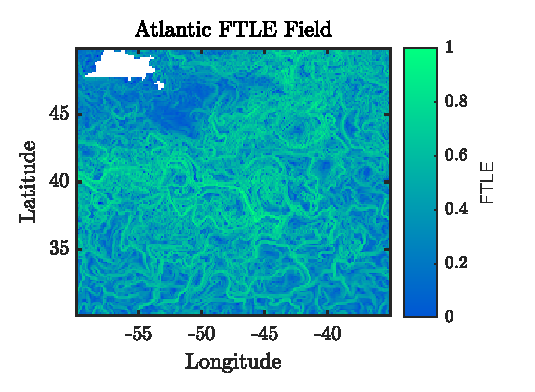
\includegraphics[scale=1]{../figures/atlantic_ftle.eps}%
	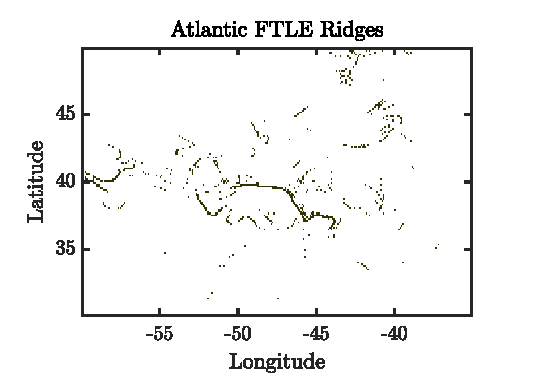
\includegraphics[scale=1]{../figures/atlantic_ftle_ridges.eps}
	\caption{Results of the FTLE diagnostic on the oceanographic data. The left-hand plot colours each initial position by the normalised FTLE value of the subsequent trajectory. The right-hand plot highlights the extracted maximising regions in black.}
	\label{fig:atlantic_ftle}
\end{center}
\end{figure}

Figure \ref{fig:atlantic_ftle} plots the FTLE field and the corresponding extracted ridges. The ridges are extracted by taking the trajectories with an FTLE value at least 80\% the maximum (i.e. values larger than 0.8 when normalised). Under the FTLE definition of LCSs, the extracted ridges are a coherent structure while the remaining trajectories make up the incoherent background flow. We convert the extracted ridges to a partition with two clusters accordingly: one corresponding to these maximising regions, and another corresponding to the remaining incoherent background. Hence, using our clustering framework, we have \(K_{\text{FTLE}} = 2\) and a \(44279\times 2\) membership matrix \(M_{\text{FTLE}}\). The maximising regions appear to loosely reflect the Gulf Stream and the surrounding flow, possibly suggesting that the Stream is a flow barrier. A more sophisticated ridge extraction technique may better distinguish this, but for our purposes we take the extracted regions as an LCS.

\begin{figure}
\begin{center}
	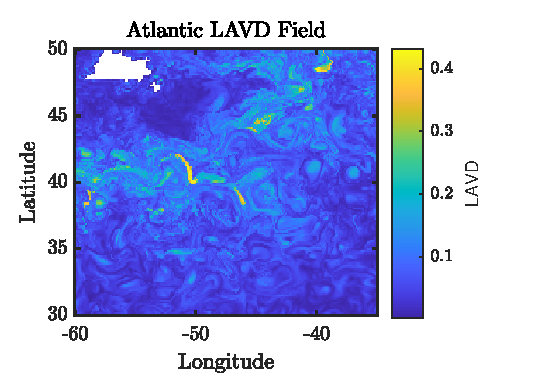
\includegraphics[scale=1]{../figures/atlantic_lavd.eps}%
	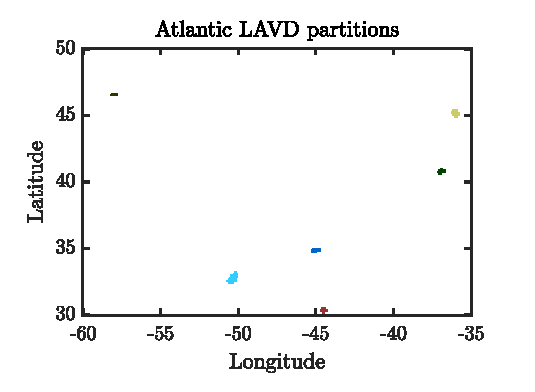
\includegraphics[scale=1]{../figures/atlantic_member_lavd.eps}
	\caption{Results of the LAVD diagnostic on the oceanographic data. The left-hand plot colours each initial position by the normalised LAVD value of the subsequent trajectory. The right-hand plot highlights the extracted vortices by colouring each.}
	\label{fig:atlantic_lavd}
\end{center}
\end{figure}

Figure \ref{fig:atlantic_lavd} shows the LAVD field and the corresponding extracted vortices. The vortices are extracted using the algorithm written and implemented by \cite{haller_2016_lavd}. There are 6 small vortices, each of which is a cluster under our clustering framework. The remaining trajectories which are not assigned to a vortex are assigned to one cluster representing incoherent background flow. We therefore have \(K_{\text{LAVD}} = 7\) and a \(44279\times 7\) membership matrix \(M_{\text{LAVD}}\). Note that the exact number of vortices extracted can be changed by modifying numeric parameters, but in all cases we extract small vortices and no larger scale structure. 



\subsection{Trajectory Clustering}
\begin{figure}%{r}{0.5\textwidth}
\begin{center}
	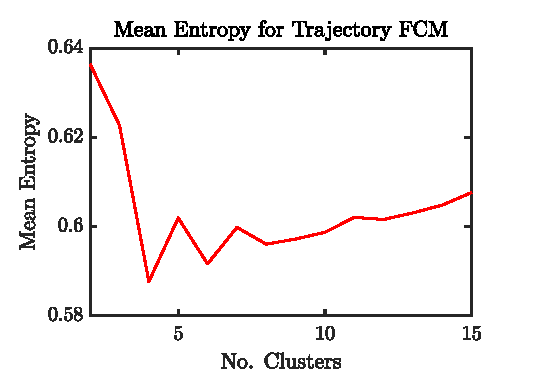
\includegraphics[scale=1]{../figures/atlantic_ent_traj.eps}%
	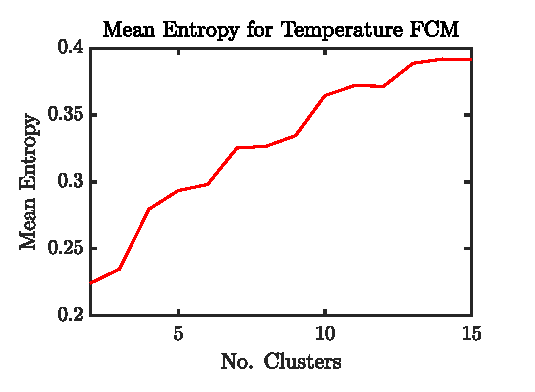
\includegraphics[scale=1]{../figures/atlantic_ent_temp.eps}
	\caption{Mean classification entropy for each number of clusters, when applying FCM to the trajectories (left) and temperature measurements (right).}
	\label{fig:ent_traj_temp}
\end{center}
\end{figure}

We also partition the trajectories using fuzzy \(c\)-means, which clusters the trajectories based on their proximity to each other. We use the fuzzifier value \(m = 2\), which is a common choice in most applications. Figure \ref{fig:ent_traj_temp} plots the mean classification entropy for FCM applied to the trajectory data, varying the number of clusters from 2 to 15. We accordingly take the optimal number of clusters to be 4. We therefore have \(K_{\text{FCM}} = 4\) and a \(44279\times4\) membership matrix \(M_{\text{FCM}}\).

\begin{figure}
\begin{center}
	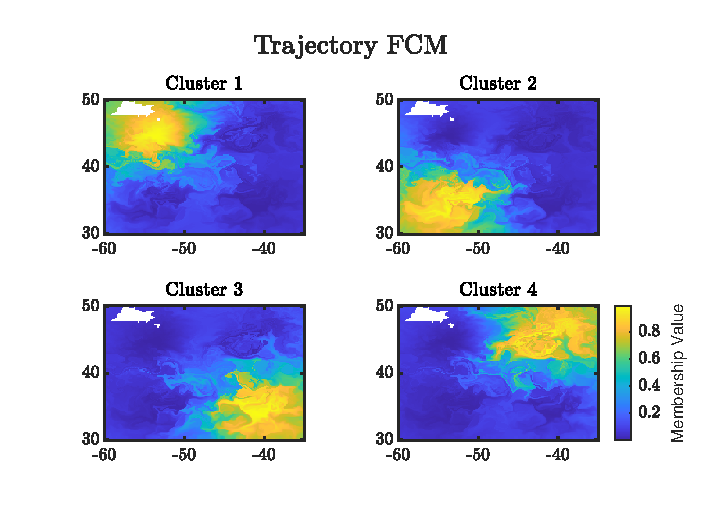
\includegraphics[scale = 1.5]{../figures/atlantic_member_traj.eps}
	\caption{Each initial position of a trajectory, coloured by membership value for each cluster using FCM on the trajectory positions.}
	\label{fig:atlantic_traj_member}
\end{center}
\end{figure}

For each cluster, Figure \ref{fig:atlantic_traj_member} colours the initial positions in \(D\) by the membership values of the subsequent trajectories. The clusters divide the trajectories into four quadrants of approximately equal size. However, this clustering only highlights a limited amount of coherency; in particular, no cluster corresponds to the Gulf Stream. 


\subsection{Temperature Clustering}
The oceanography data also includes sea surface temperature measured daily at each point on the spatial grid. It has been shown that variables such as temperature which evolve alongside a fluid flow can reflect LCSs in the fluid, or suggest their own structure \citep{balasuriya_2018_glcs}. We can therefore use this data to partition the flow and compare with other partitions in our clustering framework. This will demonstrate the flexibility of the framework in handling extensions of Lagrangian notions of coherency. Figure \ref{fig:atlantic_temp} plots the SST field on 25 June, 2018. We see the Gulf Stream is reflected in the temperature field, including the initial narrow stream and the widening and loss of coherency.

\begin{wrapfigure}{r}{0.5\textwidth}
%\vspace{-20mm}
\begin{center}
	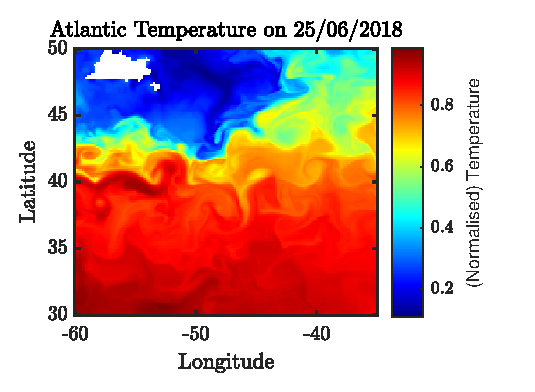
\includegraphics[scale = 1]{../figures/atlantic_temp.eps}
	\caption{Sea surface temperature field at each sampling point on 25 June, 2018, normalised to lie within \([0,1]\).}
	\label{fig:atlantic_temp}
\end{center}
\end{wrapfigure}
In order to ensure we maintain a Lagrangian perspective of the flow, we consider the temperature along each trajectory. At each time step and position at which a trajectory is sampled, we take the (Eulerian) SST at that point in space and time. This results in a temperature measurement for each sampled position along each trajectory in \(D\). This is justified by an convection-diffusion model of temperature evolution, which is often used to model such a field. We assume that temperature is simultaneously advected by the flow, which corresponds to particle trajectories, and diffused to nearby regions. By measuring the temperature field along each trajectory, we therefore gain some insight into this process. This approach also ensures that we consider temperature as a Lagrangian quantity. To partition the set of trajectories, we apply fuzzy \(c\)-means clustering on the temperature measurements along each trajectory. We again use the fuzzifier value \(m = 2\). We take 3 clusters, which by manual inspection best captures the Gulf Stream structure while still having the second-smallest mean entropy for configurations with up to 15 clusters, evidenced by Figure \ref{fig:ent_traj_temp}. Under our clustering framework, this gives \(K_{\text{Temp}} = 3\) and a \(44279\times3\) membership matrix \(M_{\text{Temp}}\).

\begin{figure}
\begin{center}
	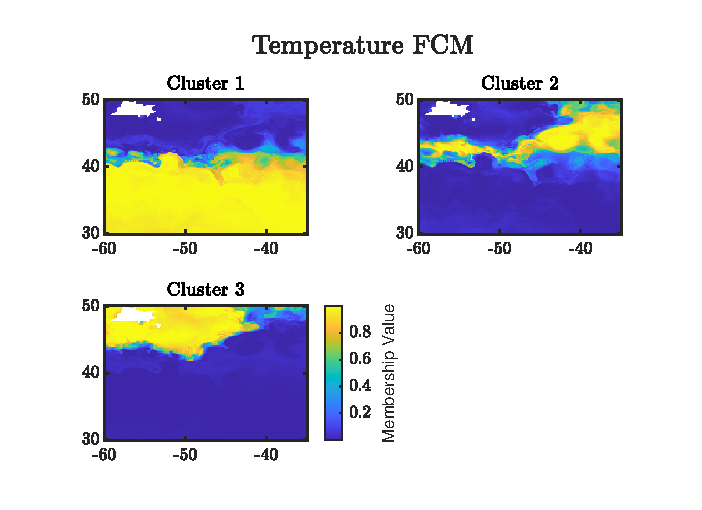
\includegraphics[scale = 1.5]{../figures/atlantic_member_sst.eps}
	\caption{Each initial position of a trajectory, coloured by membership value for each cluster using SST measurements.}
	\label{fig:atlantic_sst_member}
\end{center}
\end{figure}

Figure \ref{fig:atlantic_sst_member} plots the membership values of initial points for each cluster. Cluster 2 appears to represent the Gulf Stream and the loss of coherency towards the east of the region of interest. The remaining two clusters, Clusters 1 and 3, primarily correspond to the regions of the flow north and south of Cluster 2. This partitioning highlights the Gulf Stream and nearby trajectories as a flow barrier. 





\subsection{Consensus Clustering}
We have four basic partitions of the flow domain which have been obtained via different methods, described by the membership matrices \(M_{\text{FTLE}}, M_{\text{LAVD}}, M_{\text{FCM}}, M_{\text{Temp}}\). We now apply fuzzy consensus clustering to combine these partitions into one clustering of the flow, which ideally contains all of the highlighted structures or suggests new coherency.

\begin{figure}
\begin{center}
	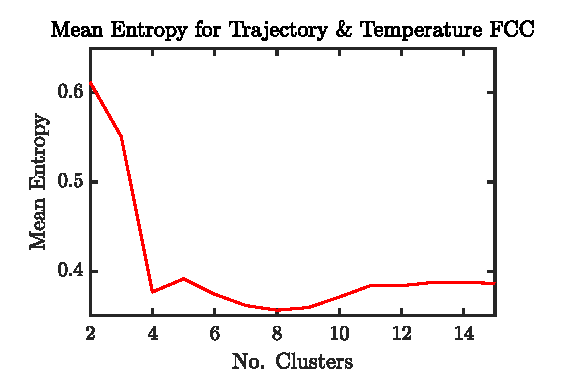
\includegraphics[scale = 0.98]{../figures/atlantic_ent_trajtemp.eps}%
	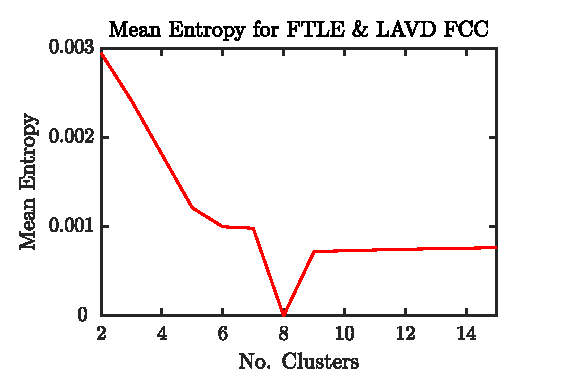
\includegraphics[scale=0.98]{../figures/atlantic_ent_ftlelavd.eps}
	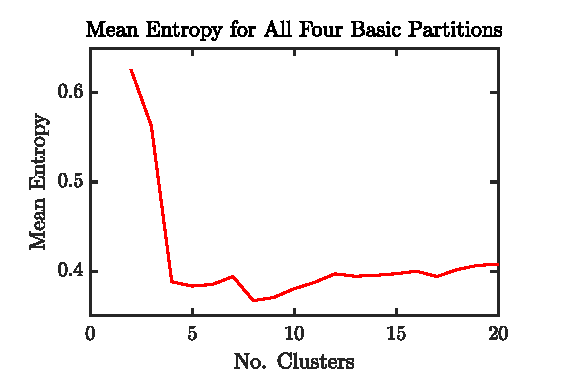
\includegraphics[scale=0.98]{../figures/atlantic_ent_all4.eps}
	\caption{Mean classification entropy for applications of FCC varying the number of clusters. Clockwise from top left, the clusters are created by combining the trajectory and temperature clusters, the FTLE ridges and LAVD vortices, and all four basic partitions. We include the mean entropy up to 20 clusters for the consensus of all four partitions, in order to explore if a larger number of clusters results in a better consensus.}
	\label{fig:cons_ents}
\end{center}
\end{figure}

We take the fuzzifier value \(m = 2\), which ensures that cluster fuzziness is consistent with the basic partitions derived using FCM. We also take equal weights for each basic partition so that each contributes equally to the final consensus. In order to select the number of clusters, we apply FCC in each case varying the number of clusters from 2 to 15. For each clustering, we calculate the mean classification entropy according to \eqref{eqn:ent} and select the number of clusters which gives the minimum value. Figure \ref{fig:cons_ents} plots the mean entropy for each combination of basic partitions that we consider.


\subsubsection{Trajectories \& Temperature}
\begin{figure}
\begin{center}
	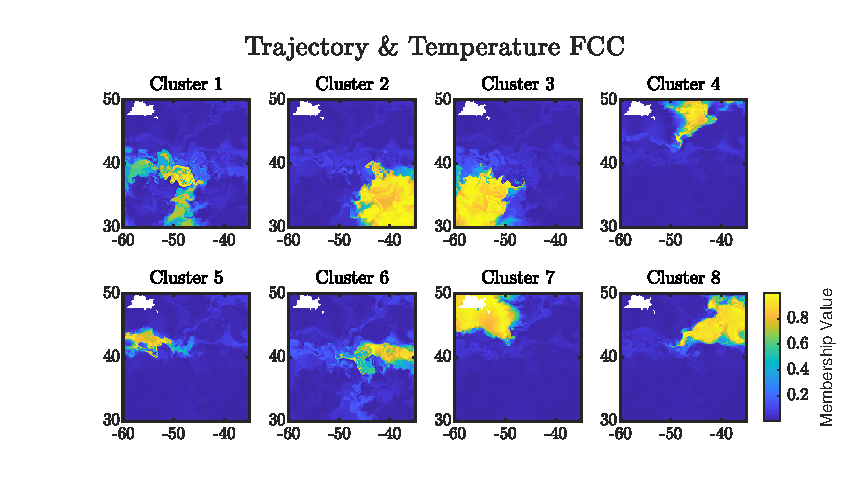
\includegraphics[scale = 1.3]{../figures/atlantic_member_trajtemp.eps}
	\caption{Membership values for the consensus clustering of partitions derived using trajectories and temperature measurements.}
	\label{fig:member_cons_trajtemp}
\end{center}
\end{figure}

We first apply the FCC algorithm to combine the partitions derived by using FCM applied to the trajectories and temperature data, i.e. the membership matrices \(M_{\text{FCM}}\) and \(M_{\text{Temp}}\). From Figure \ref{fig:cons_ents}, the minimum mean entropy occurs at \(K = 8\) clusters, so we take this as the optimal number of clusters. Figure \ref{fig:member_cons_trajtemp} plots the subsequent membership values for each cluster.

The three clusters present in the temperature basic partition (in Figure \ref{fig:atlantic_sst_member}) are divided into smaller clusters according to those produced using the trajectories (in Figure \ref{fig:atlantic_temp}). The Gulf Stream is no longer highlighted by only one cluster, but instead we see several clusters (Clusters 2, 5, 6 and 8) which contain parts of the Stream region. We see that Cluster 7 corresponds to the same northern region of the flow which Cluster 1 in the original trajectory clustering (Figure \ref{fig:atlantic_traj_member}) represented. However, the boundary is more clearly defined with less uncertainty (i.e. membership values closer to 0 or 1). We see similar results with Clusters  2 and 3, which correspond to Clusters 2 and 3 in Figure \ref{fig:atlantic_traj_member}. The remaining clusters that contain parts of the Gulf Stream may be providing more insight into the sub-structure within the Stream. Hence, the addition of a partition derived using the temperature field has improved the trajectory clusters by highlighting smaller regions, better distinguishing the Gulf Stream and improving the crispness of clusters.


\subsubsection{FTLE \& LAVD}
\begin{figure}
\begin{center}
	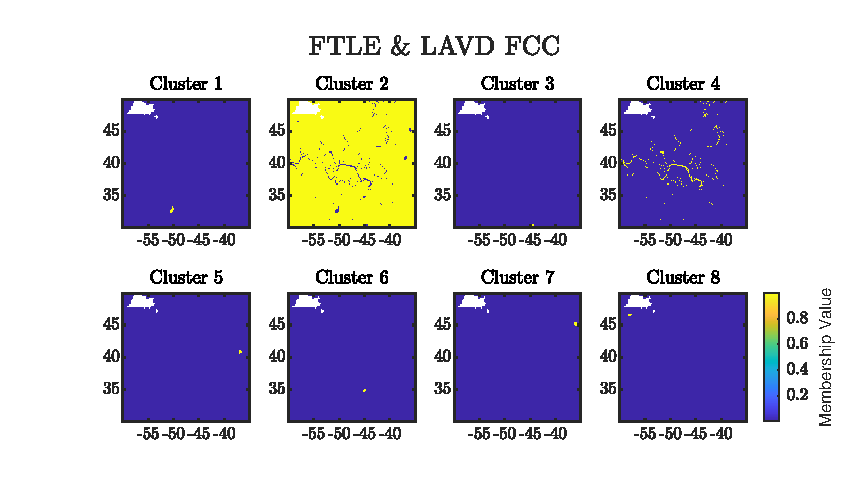
\includegraphics[scale = 1.3]{../figures/atlantic_member_ftlelavd.eps}
	\caption{Membership values for the consensus clustering of partitions derived using FTLE ridges and LAVD vortices.}
	\label{fig:member_cons_ftlelavd}
\end{center}
\end{figure}

The FTLE and LAVD fields characterise contrasting aspects of the flow: the FTLE measures stretching, whereas the LAVD quantifies rotation. Accordingly, the flow is partitioned into different structures, shown in Figures \ref{fig:atlantic_ftle} and \ref{fig:atlantic_lavd} and described by membership matrices \(M_{\text{FTLE}}\) and \(M_{\text{LAVD}}\). We therefore apply FCC to combine these two partitions into one clustering. From Figure \ref{fig:cons_ents}, the minimum mean entropy occurs with \(K = 8\) clusters, so we use this many clusters. Figure \ref{fig:member_cons_ftlelavd} plots the subsequent membership values for each cluster.

Each cluster other than Cluster 2 represents an individual structure extracted using the FTLE and LAVD methods. Clusters  1, 3, 5, 6, 7 and 8 each correspond to a vortex extracted using the LAVD field, while Cluster 4 consists of the FTLE ridges. Cluster 2 corresponds to the remaining region of flow, which we interpret as incoherent background flow.

Each membership value is either 0 or 1, so this clustering is hard. This is a special case of the FCC algorithm, where we combine non-overlapping hard clusters into a sufficient number of consensus clusters. Each cluster in the basic partitions is reconstructed by the FCC algorithm. Since the basic partitions are hard and non-overlapping, the resulting consensus is also hard, despite setting \(m > 1\). The mean entropy is accordingly 0, since there is no uncertainty in cluster assignment. This is an intuitive result and verifies that FCC can produce the obvious consensus of non-overlapping, hard clusters.



\subsubsection{All Partitions}
\begin{figure}
\begin{center}
	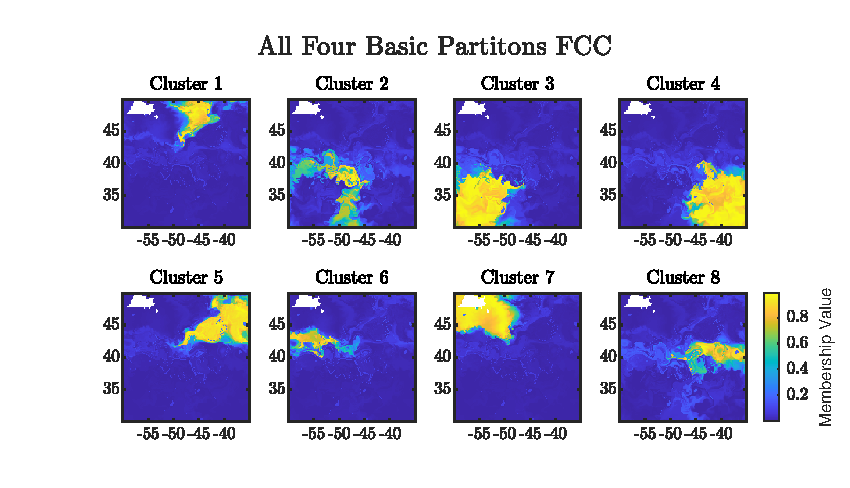
\includegraphics[scale=1.3]{../figures/atlantic_member_all.eps}
	\caption{Membership values for the consensus clustering of all four basic partitions, with 8 clusters.}
	\label{fig:member_cons_all}
\end{center}
\end{figure}
As a final example, we apply FCC to combine all four basic partitions: the trajectory and temperature clusters obtained using FCM, and the structures extracted using the FTLE and LAVD fields. From Figure \ref{fig:cons_ents}, the minimum mean entropy occurs with \(K = 8\) clusters. Figure \ref{fig:member_cons_all} plots the membership values for each trajectory. 

The resulting clusters are almost identical to those obtained by combining only the trajectories and temperature measurements, in Figure \ref{fig:member_cons_trajtemp}. No clusters correspond directly to the smaller scale structure defined by the FTLE and LAVD ridges. Instead, these structures are spread across all 8 clusters, so that each cluster contains a region of low probability corresponding to these structures. This may be due to an insufficient number of clusters, or adjusted weightings to favour the FTLE and LAVD basic partitions may rectify this issue.

We therefore also consider the same FCC set-up, but with 17 clusters, which is a local minimum of mean entropy with respect to the number of clusters. Figure \ref{fig:extra_cons} in Appendix \ref{app:cons} plots the resulting membership values. We see that the large-scale structure extracted by the trajectory and temperature clusters are split into finer regions with the addition of the small-scale structure given by the FTLE and LAVD partitions. For example, Cluster 16 appears to have isolated the barrier between the northern region of the flow and the Gulf Stream, likely due to the FTLE partitioning. Clusters 11 and 15 may have isolated the two main components of the Gulf Stream; the narrow emanation towards the east of the flow domain and the subsequent widening, respectively. However, several of the clusters are difficult to relate directly to classical coherent structures, and there is much overlap between clusters, resulting in a noisier picture than we saw with 8 clusters.

The two different results using 8 and 17 clusters demonstrates that our method for selecting the number of cluster is not necessarily ideal. Despite 8 clusters being optimal by our adopted method, we see that a larger number of clusters better represents all four basic partitions.


\section{Conclusion}
We have proposed a clustering framework as a means of comparing multiple partitions of the same set of Lagrangian trajectories. By describing each partition with a membership matrix, we disregard the means for which the partition was derived, allowing for equal comparison. We then apply fuzzy consensus clustering to combine these partitions into one and demonstrate this algorithm with an example using oceanographic data. This example demonstrated that the FCC algorithm is able to combine features from different partitions of the same flow, to enhance and suggest new structure. While the clustering just using the trajectory measurements was unable to distinguish the Gulf Stream as a cluster, the temperature clusters produced a clear picture of the Stream as a flow barrier. Combining the two with FCC improved the trajectory cluster by distinguishing finer structure including the Stream, and producing crisper clusters. We also saw an obvious result when combining hard and non-overlapping basic partitions, where we produced one clustering containing all small-scale structure derived from the FTLE and LAVD methods. However, the number of clusters must be user-specified and had impact on how well-represented the basic partitions were in the final consensus. This was evident when using FCC to combine all four basic partitions, where the optimal number of clusters according to an entropy-based optimisation approach was not sufficient to reflect all structure highlighted by each basic partition. Developing a method for determining the optimal number of partitions, as well as tuning other parameters in the algorithm, therefore provides an avenue for future work. Moreover, there is an opportunity to gain a more rigorous theoretical understanding of the clustering framework and FCC approach by implementing it on a simple toy model, such as the double gyre or Bickley jet, and comparing results with other LCS studies. Nonetheless, the framework provides a promising foundation for distinguishing new LCSs in a given flow.




\clearpage
\bibliographystyle{agsm}

\bibliography{../notes/lcs_bib.bib}

\clearpage
% Appendices go here as required

\begin{appendices}
\section{Algorithms}

\subsection{Fuzzy \(c\)-means Clustering}\label{app:fcm}
Algorithm \ref{alg:fcm} details the fuzzy \(c\)-means clustering algorithm, as adapted  by \cite{froyland_2015_fuzzy} for time-sampled trajectory data.

\begin{algorithm}[H]
Let \(\bm{C}_1(t_i), \hdots, \bm{C}_c(t_i)\) denote the centres at time \(t_i\), for \(i = 0,1,\hdots, n_t\), to be consistent with our notation. Let \(M_{lk}\) denote the membership value of the \(l\)th trajectory (with initial position \(\bm{x}_0^{(l)}\)) to the \(k\)th cluster (defined by centre \(\bm{C}_k\). For the \(l\)th time-sampled trajectory in \(D\), let \(\bm{X}_i \in \R^{d\times n_t}\) denote the concatenation of all dimensions along the trajectory. Recall that \(d\) is the dynamic metric \eqref{eqn:dynmet}, with the Euclidean distance metric \(\rho\).
\begin{enumerate}
\item Initialise membership values \(M_{lk}\) either randomly or via step 3 based on an initial seeding of \(K\) centres.
\item Calculate centres: for \(i = 0,1,\hdots, n_t\) and \(k = 1,\hdots,c\),
\[
\bm{C}_k(t_i) = \frac{\sum_{l=1}^{n}{\left(M_{lk}\right)^m \bm{x}^{(l)}\left(t_i\right)}}{\sum_{l=1}^n{\left(M_{lk}\right)^m}}.
\]
\item Update membership values: for \(k = 1,\hdots,c\), \(l = 1\hdots,n\),
\[
M_{lk} = \frac{1/d\left(\bm{x}^{(l)}_0, \bm{C}_k(t_0)\right)^{2/(m-1)}}{\sum_{j=1}^{K}{1/d\left(\bm{x}^{(l)}_0, \bm{C}_j(t_0)\right)^{2/(m-1)}}}.
\]

\item Evaluate the objective function
\[
\sum_{k=1}^{K}{\sum_{i=1}^{n}{M_{lk}^m d\left(\bm{x}_0^{(l)},\bm{C}_k(t_0)\right)^2}}.
\]
If the change from the previous value of the objective function is less than a fixed threshold, terminate. Otherwise, store the new value and go to step 2.
\end{enumerate}
\caption{Fuzzy \(c\)-means algorithm adapted for trajectory clustering \cite{froyland_2015_fuzzy}.}
\label{alg:fcm}
\end{algorithm}

\vspace{5mm}
\subsection{Fuzzy Consensus Clustering}\label{app:fcc}
Algorithm \ref{alg:fcc} details the fuzzy consensus clustering proposed by \cite{wu_2017_fcc}, adapted to the clustering framework notation. Note that the algorithmic framework additionally requires the specification of some convex function \(\phi(\bm{x})\) which maps vectors in \(\R^k\) of arbitrary dimension \(k\) to values in \(\R\). This function ultimately defines the similarity metric for comparing the multi-membership values of trajectories to cluster centres. There are many different choices for this function \citep{wu_2017_fcc}, but we elect to use the standard choice of the Euclidean distance metric \(\phi(\bm{x}) = \norm{\bm{x}}^2\).
\begin{algorithm}[H]
\caption{The fuzzy consensus clustering algorithm \cite{wu_2017_fcc}, with notation adapted to match that used in this paper.}

Through the iterative process, the \(K\) centres defining each cluster are stored as the vectors \(\bm{v}_1,\hdots,\bm{v}_K \in\sum_{i=1}^{r}{K_i}\). Let \(v_k^{(i)}\) denote the sub-vector of \(\bm{v}_k\) with \(K_i\) elements corresponding to the clusters of the \(i\)th basic partition. We can then write \(\bm{v}_k = \begin{bmatrix}v_k^{(1)} & v_k^{(2)} & \cdots & v_k^{(r)}\end{bmatrix}\). Let \(M_{l\cdot}^{(i)}\) denote the \(l\)th row of the membership matrix \(M^{(i)}\).  Define the weighted distance function \(d: \mathcal{Y}\times \R^{\sum_{i=1}^{r}{K_i}} \to \R\) by
\[
d(\bm{y}_l, \bm{v}_k) = \sum_{i=1}^{r}{w_i\norm{M_{l\cdot}^{(i)} - v_k^{(i)}}}.
\]
The FCC algorithm is as follows:
\begin{enumerate}
	\item Randomly initialise an \(n\times K\) matrix \(M\) of membership values, ensuring each row sums to 1, i.e. for every \(l = 1,\cdots, n\) we have that \(\sum_{k=1}^{K}{M_{lk}} = 1\).
	\item Update the centre vectors via
	\[
	v_k^{(i)} = \frac{\sum_{l=1}^{n}{\left(M_{lk}\right)^m}M_{l\cdot}^{(i)}}{\sum_{l'=1}^{n}{\left(M_{l'k}\right)^m}}.
	\]
	
	\item Update the membership values via
	\[
	M_{lk} = \frac{d\left(\bm{y}_l, \bm{v}_k\right)^{-1/(m-1)}}{\sum_{k' = 1}^K{d\left(\bm{y}_l, \bm{v}_{k'}\right)^{-1/(m-1)}}},
	\]
	for each \(l = 1,\hdots,n\) and \(k = 1,\hdots,K\).
	
	\item Evaluate the objective function
	\[
	J(M,\bm{v}_1, \hdots, \bm{v}_K) = \sum_{k=1}^{K}{\sum_{l=1}^n\left(M_{lk}\right)^m d(\bm{y}_l, \bm{v}_k)}.
	\]
	If the change from the previous value is less than a specified threshold, terminate. Otherwise, store the value and go to step 2. 
	
\end{enumerate}
\label{alg:fcc}
\end{algorithm}

%\clearpage
%\section{Pre-processing of Oceanographic Data}\label{app:ocean}
%The ocean measurements consisted of meridional and zonal current velocities (in m.s\(^{-1}\)) and sea surface temperature (in degrees Celsius), measured daily at each point on a spatial grid of resolution \(1/12\ddeg\) in the latitudinal and longitudinal directions. To perform LCS anlaysis, we needed to generate trajectories from this Eulerian velocity data. To integrate trajectories, the velocity data was converted to the same spatial units as the grid. The data is processed using the WGS-84 model of the Earth \citep{wgs84}, where the shape of the Earth is approximated as an ellipsoid with major axis radius \(\) and eccentricity \(\). We therefore convert velocities from \(m.s^{-1}\) to \(\,^{\circ}.s^{-1}\) via
%\begin{align*}
%u_{\,^{\circ}} & = \\
%v & = 
%\end{align*}
%where \(\text{lat}\) is latitude.
%
%The flow domain \(\Omega\) was chosen so that no particles leave the larger data domain. This presents any complications resulting from the need to extrapolate the velocity data.
%
%To generate trajectories, a uniform grid of \(300\times 150\) initial positions was created, and for each \eqref{eqn:trajode} was solved numerically using the \verb|ode45| function in \textsc{Matlab}, which implements the Rune-Kutta Dormand–Prince method for numerically solving ODEs. This required interpolation of the velocity field where measurements were not provided, which was done via a cubic interpolant and the \verb|griddedInterpolant| function in \textsc{Matlab}. Any trajectories which were initialised on the land were then omitted from the subsequent analysis.
%
%The temperature data was similarly interpolated, 
%
%
%
%
%
%
%
%\clearpage
%\section{Numerical Considerations}
%In order to calculate the FTLE and LAVD fields from the oceanographic data, we were required to numerically approximate several derivatives and integrals related to the flow. To approximate the Cauchy-Green tensor, following the approach of \cite{haller_2015_lcs} we use the following star-grid finite difference approximation
%\[
%\nabla F_{t_0}^{t}(\bm{x}_0) \approx \begin{pmatrix}
%	\frac{x(t; \,\bm{x}_0 + \delta x\bm{i}) - x(t; \,\bm{x}_0 - \delta x\bm{i})}{2\,\abs{\delta x}} & \frac{x(t; \,\bm{x}_0 + \delta y\bm{j}) - x(t; \,\bm{x}_0 - \delta y\bm{j})}{2\,\abs{\delta y}} \\
%	\frac{y(t; \,\bm{x}_0 + \delta x\bm{i}) -y(t; \,\bm{x}_0 - \delta x\bm{i})}{2\,\abs{\delta x}} & \frac{y(t; \,\bm{x}_0 + \delta y\bm{j}) - y(t; \,\bm{x}_0 - \delta y\bm{j})}{2\,\abs{\delta y}} \\
%\end{pmatrix},
%\]
%where \(F_{t_0}^t(\bm{x}_0) = x(t\sc\bm{x}_0)\bm{i} + y(t\sc\bm{x}_0)\bm{j}\). 
%
%
%The LAVD calculation requires calculation of the vorticity along each trajectory, which was approximated via a centred finite difference approximation of the first derivatives. Since the flow is in \(\R^2\), the vorticity \(\bm{\omega} = \omega_3\bm{k}\) has only one non-zero component,
%\[
%\omega_3 = \dpd{v}{x} - \dpd{u}{y}.
%\]
%Using a central finite-difference approximation for each derivative, the vorticity at position \(\bm{x} \in \R^2\) at time \(t\) is approximated as
%\[
%\omega_3(\bm{x},t) \approx \frac{v(t,\bm{x} + \delta x\bm{i})}{}
%\]
%
%The spatial mean of the vorticity is then approximated using the sample mean along each trajectory at that time, i.e.
%\[
%\bar{\bm{\omega}}(t) \approx \frac{1}{n}\sum_{\bm{x}_0 \in D}{\bm{\omega}\left(F_{t_0}^{t}(\bm{x}_0), t\right)}.
%\]


\section{Additional Consensus Clustering}\label{app:cons}
\begin{figure}[H]
\begin{center}
	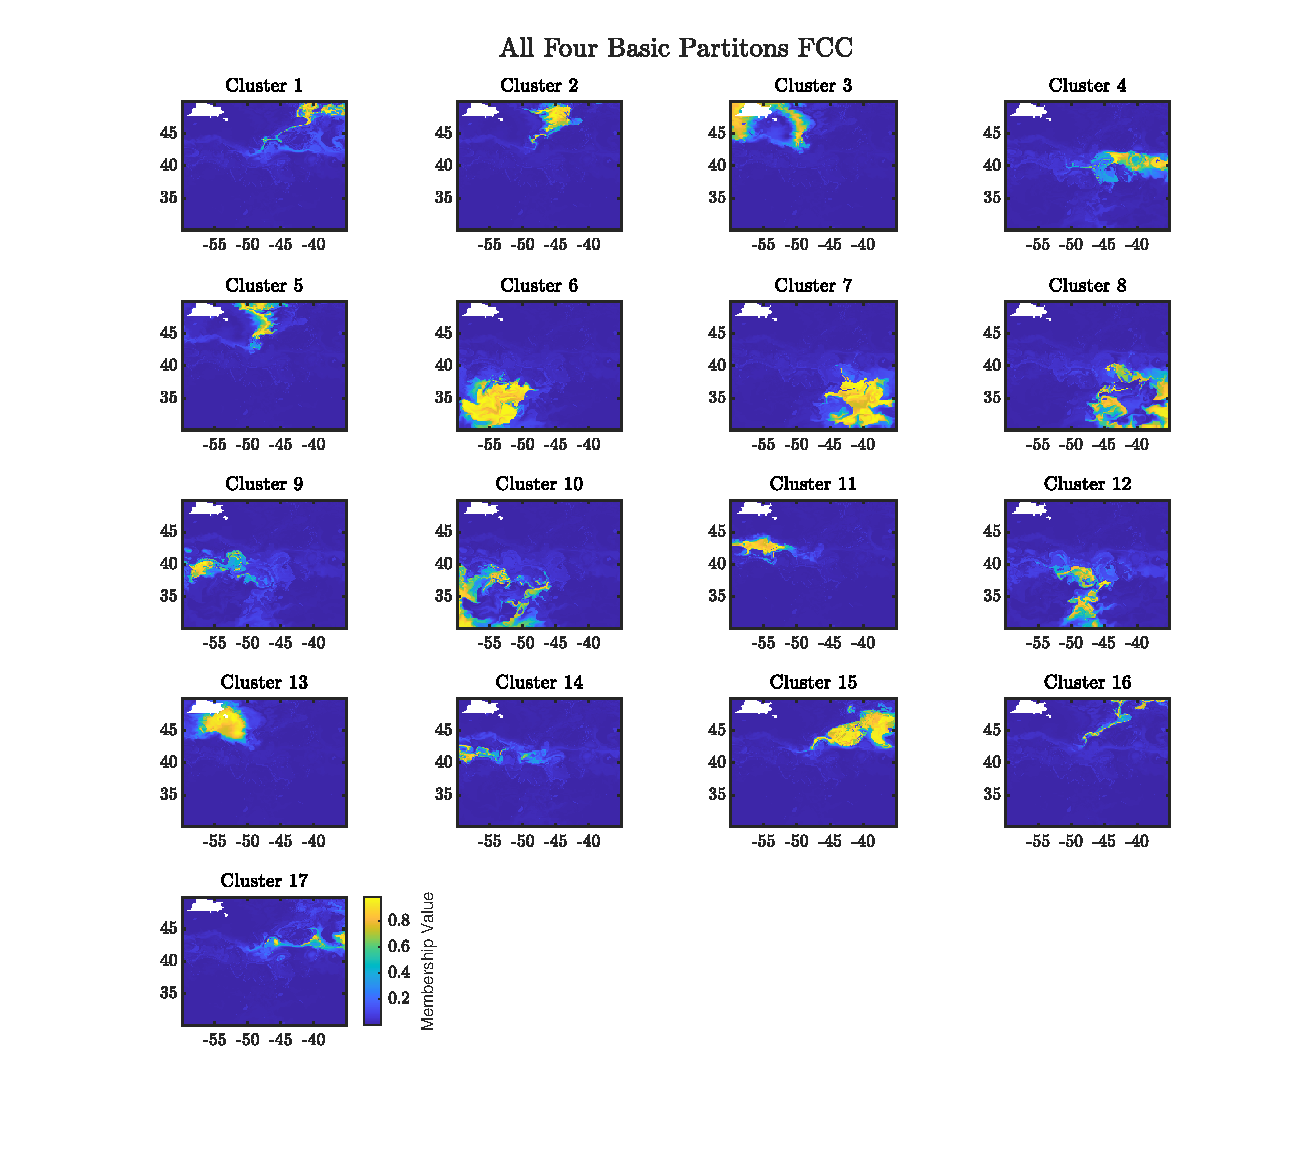
\includegraphics[width=\textwidth]{../figures/atlantic_member_all17.eps}
	\caption{Membership values for the consensus clustering of all four basic partitions, with 17 clusters.}
	\label{fig:extra_cons}
\end{center}
\end{figure}
\end{appendices}

\end{document}


